\newpage	
\def \currentAuthor {Florian Tipotsch}
	\section{Technologie für Webapp}
\begin{itemize}
	\item PHP - Für Handyapp
	\item Html - Für Handyapp 	
	\item MySql - Für Datenbanken
	\item Yii2 - Für Handyapp
\end{itemize}
	\section{Yii2}
	\subsection{Was ist Yii}
	Yii ist ein high Performance PHP Framework welches vorallem für die Entwicklung im Web2.0 eingesetzt wird. Web 2.0 fördert die user aktiv im Web mitzumachen. Diese können eigenen Beiträge erstellen und diese auf der Website anzeigen lassen.
\cite{Web2}
	\subsection{Alternativen für Yii}
	Yii kann sehr weitreichend eingsetzt werden. Mit dem richtigen Wissen und Fähigkeiten kann man alles was mit einer PHP Seite möglich ist ganz einfach in Yii2 umsetzten. Dabei gibt es auch viele Vorteile:
\begin{itemize}
\item CRUD-Creator
\item Model Generator
\item Einfache implementierung von HTML Formulare
\end{itemize}
Allerding sind Frameworks nicht Administrationsfreundlich da sie sehr viel Vorkentniss erfordern um diese richtig zu implementieren. Einfacher zu implementieren sind CMS Systeme. Es gibt sehr viele Große CMS Systeme zum Beispiel:
\begin{itemize}
\item Joomla
\item Wordpress
\item Drupal
\item Contao
\end{itemize}
Diese haben wir auch schon im Unterricht besprochen und damit Websiten erstellt. Vorteile sind vorallem die einfache implementierung und rasche einrichtung einer Website. Auch SEO wird von den CMS Systemen vereinfacht. Nachteile sind allerdings oft eingeschränkte möglichkeiten und grenzen die das CMS setzt.

Es gibt auch noch viele andere Frameworks zum Beispiel:

\subsection{Warum haben wir uns für YII2 entschieden}

Der Hauptgrund waum wir uns gegen CMS Systeme entschieden haben sind die eingeschränkten möglichkeiten die wir damit hätten. Bei YII2 können wir die gesamte Website nach unseren Bedarf zusammenstellen und auch so bearbeiten wie wir es wollen. Es war uns auch wichtig das wir nach modernen Entwurfsmustern arbeiten (hier MVC).





\newpage
\section{Gas-Sensoren}
\subsection{MQ Gas Sensoren}
Es gibt mehrer MQ Gas Sensoren zum Beispiel:
\begin{itemize}
\item {MQ2}
	Methane, Butane, LPG, smoke
\item {MQ3}
	Alcohol, Ethanol, smoke
\item {MQ4}
	Methane, CNG Gas
\item {MQ5}
	Natural gas, LPG
\item {MQ6}
	LPG, butane gas
\item {MQ7}
	Carbon Monoxide
\item {MQ8}
	Hydrogen Gas
\item {MQ9}
	Carbon Monoxide, flammable gasses
\item Mehr gibt es auf der Website: \cite{Gas}
\end{itemize}
In der Schule haben wir den MQ2 zur verfügung stehend werden wir auch von der Schule den Adafruit CCS811 bereitgestellt bekommen. Wir bedanken uns dafür vielmals.
\newline
{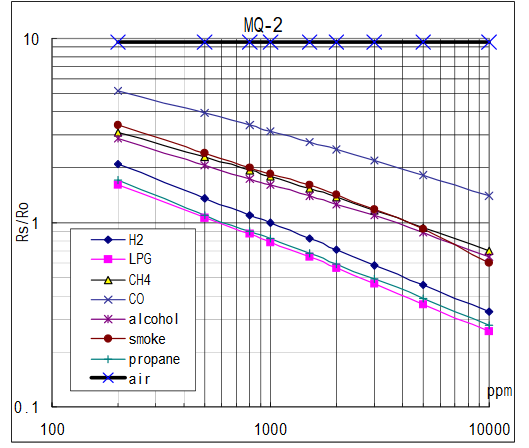
\includegraphics[width=0.8\linewidth]{figures/DatasheetMQ2.png}}{\cite{Datasheet}}
\cite{Gas}
\subsection{Adafruit CCS811}

